\section{Results}

\subsection{\textit{Nonblock} intralayer models}


% \vspace{-1.5em}
% \begin{wrapfigure}{r}{0.7\textwidth}
%     \centering
%     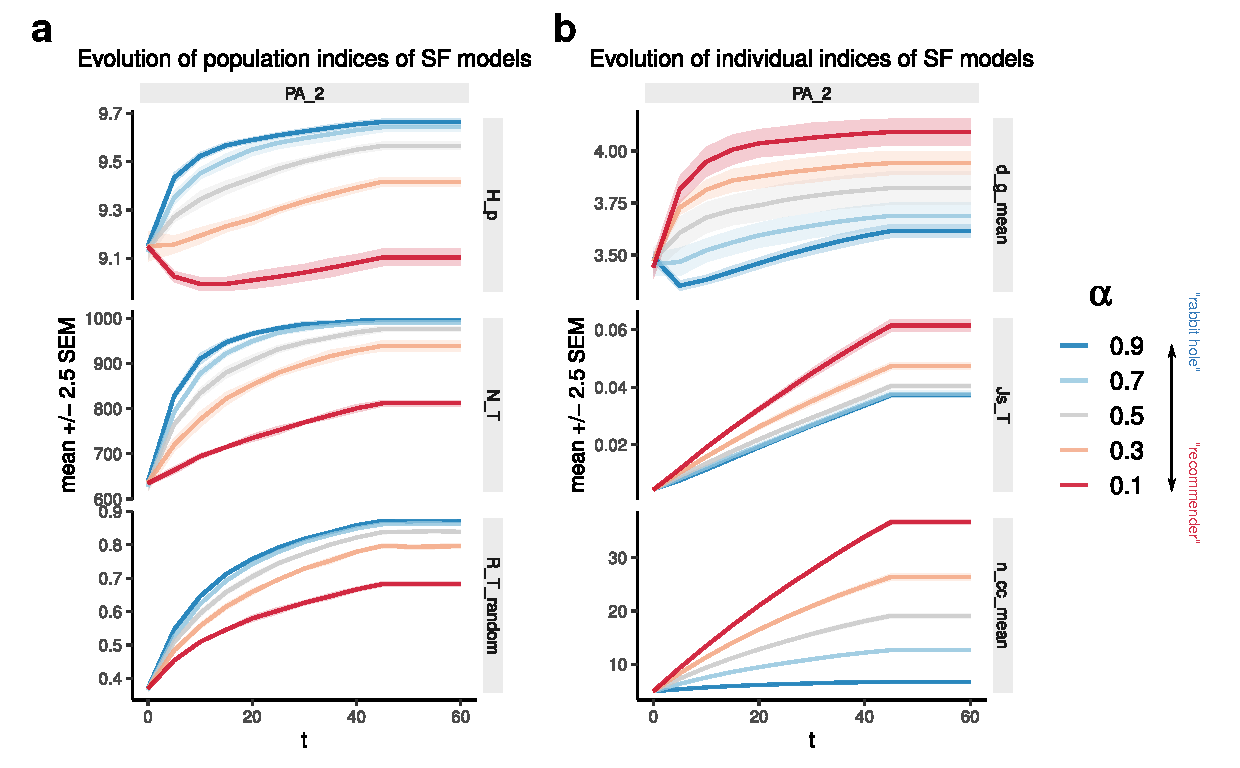
\includegraphics[width=0.7\textwidth,center]{../figures/report/Fig3.pdf}
\begin{figure}
    \centering
    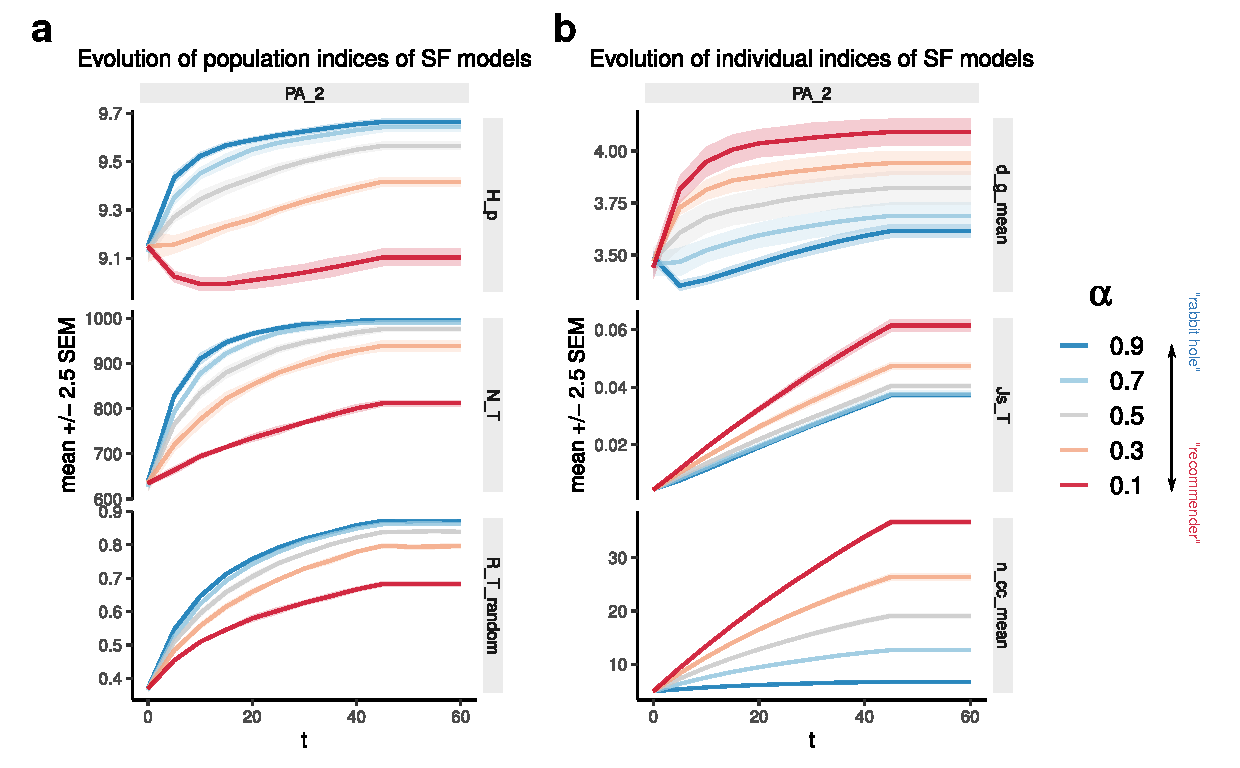
\includegraphics[width=0.7\textwidth,center]{../figures/report/Fig3.pdf}
    \caption{\label{fig:3}
    \textit{Changes of population diversity indices} (\textbf{a}) \textit{and of individual diversity indices} (\textbf{b}) \textit{of the scale-free intralayer models} ($PA_2$) \textit{due to} $\alpha$. $H_p$: topic population entropy; $N_T$: number of distinct topics; $R_T$: robustness due to random removal of agents; $d_g$: mean distance of the subset of topics that agents know; $Js_T$: Jaccard similarity of topic set between agents; $n_{\mathrm{cc}}$: number of connected components of induced subgraphs based on each agent's learnt topics. See method for detailed description.
%     \vspace{-1.5em}
    }
\end{figure}
% \end{wrapfigure}\leavevmode


The changes of the different diversity metrics for the scale-free networks ($PA_2$) are shown in \autoref{fig:3} as an example to illustrate the tradeoff effect of the ``rabbit-hole'' versus ``recommender'' probability on the population and individual diversity.

Generally, topic population diversity increases with $\alpha$ in terms of the topic entropy $H_g$ and number of topics $N_T$. Through learning/discovery through time, low $\alpha$ could still achive better population diversity. However, it does not seem likely for the worst case considered here, where entropy does not even increase pass its initial value. The initial decrease of $H_g$ when $\alpha = 0.1$ is because the agents start learning from each other, hence temporarily creating bias towards some topics, leading to decrease of entropy. It must be noted here that the entropies are already high initially due to initialization. However, taking the trends of both $N_T$ and $H_g$ into account, it is confident to say that higher $\alpha$ improves topic population diversity. Additionally, higher $\alpha$ leads to more robust retainment of the topics under random agent removal (i.e. higher $R_T$).

On the other hand, topic individual diversity usually decreases based on the chosen metrics. Increased $\alpha$ leads to decreased mean learnt topics distance $d_g$ and number of components $n_{\mathrm{cc}}$ in the induced subgraphs. Intuitively, lower $\alpha$ would allow the agents to access topics out of their comfort zone easier, hence their own subgraph of topics tend to be more generalist, whereas higher $\alpha$ leads to more specialization. Lastly, at the local level $Js_T$, lower $\alpha$ leads to more similarity between neighbors, hence lower local diversity.

These trends are quite consistent across different considerations of non-block models (\autoref{fig:4}). Increasing in $\alpha$ leads to higher topic population diversity ($N_T, H_P$), robustness ($R_T$) and local diversity $Js_T$. On the other hand, such increases tend to result in loss of topic individual diversity ($d_g$, $n_cc$). When taking into account degree-dependent initialization strategies (\autoref{supp:1}), favoring more obscure topics leads to the same trend as random initialization, though small effects when $\alpha$ is small (first 2 rows in \autoref{supp:3}). However, initially favoring more popular topics actually would be detrimental generally across all population, local and diversity, especially for those networks generated by preferential attachments (PA) models, possibly because the learning gets ``stuck'' around the nodes around those population ones (last row in \autoref{supp:3})

\begin{figure}[H]
    \centering
    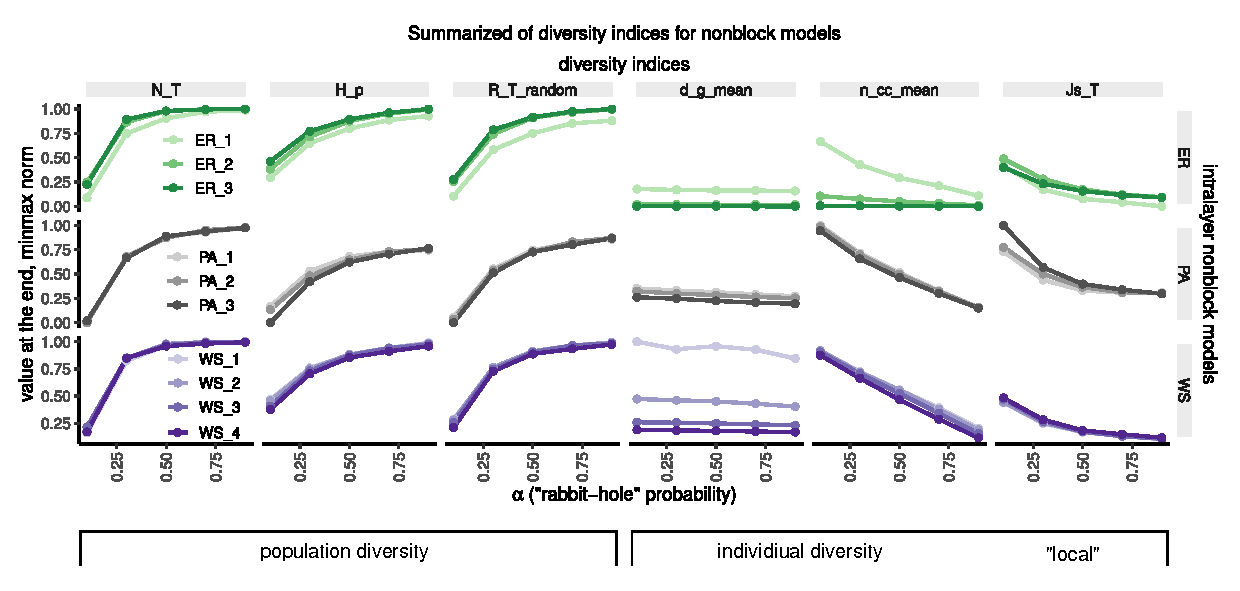
\includegraphics[width=0.95\textwidth,center]{../figures/report/Fig4.pdf}
    \caption{\label{fig:4}
    \textit{Summary of population and individual diversity indices due to $\alpha$, across different nonblock models (with random initialization)}. The values here are at the end of the simulation, and min-max normalized within each metric (panels from left to right, see text and \autoref{fig:3} for description of these different definitions). The different models are shown by colors and panels from top to bottom (see also \autoref{fig:2} for correspondence of colors).
    }
\end{figure}

In summary, in non-block intralayer models, higher $\alpha$ leads to higher topic diversity in a local and population context, but lower individual topic diversity. Initialization favoring more popular topics seems to have a negative effect on these different metrics.


\subsection{\textit{Block} intralayer models and topic group diversity}

As real-world networks usually contain communities within them, I use the stochastic block models (SBM) to observe how diversity indices change due to $\alpha$ and network modularity. Generally, the trends for population diversity and robustness during the simulation are similar from previously discussed (\autoref{supp:4}). The trends as a function of model modularity do not seem to differ much either (however the final values do show some differences, and will be discussed later). Looking at the group population entropy $H_{\mathrm{gp}}$ (\autoref{fig:5}a), only when the networks are less modular do such values show a difference, albeit very small. In particular, only when $\alpha$ is very low that such a disadvantage could be visibly inspected (very low $\alpha$ basically leads to learning in groups).

In the individual perspective (\autoref{fig:5}b), group modularity actually helps with diversity indices $d_g$ and $n_{\mathrm{cc}}$, possibly because there are few long-range links. The trends for local diversity are roughly similar and not affected much by group modularity. However, their final values do show some difference (will be discussed later). Additionally, instead of only looking at topic group diversity in the population sense, one could also inspect it in the individual perspective. On average (panel a, top), for more modular intralayer networks, lower $\alpha$ benefits topic group diversity in the agents, because the agents would have higher chance to learn out of their own comfort zone, especially if their initial topics belong to the same groups. With decreasing group modularity, these differences between $\alpha$ do not seem to matter any more.

\begin{figure}[!ht]
    \centering
    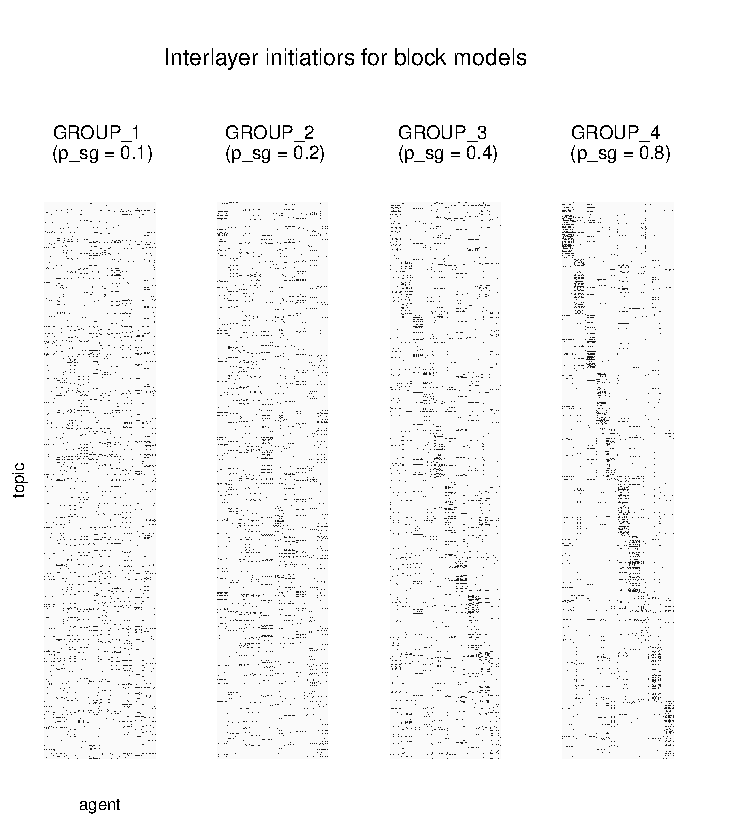
\includegraphics[width=\textwidth]{figures/FigS2.pdf}
    \caption{\label{fig:5}
    \textit{Changes of group diversity indices} (\textbf{a}) \textit{and of individual diversity indices} (\textbf{b}) \textit{of the stochastic block intralayer models} \textit{due to} $\alpha$. $H_{\mathrm{gi}}$: topic individual entropy; $H_{\mathrm{gp}}$: topic population entropy. From left to right, the models are designed to have decreasing modularity (see \ref{fig:2}). See also \ref{fig:3} and text for descriptions of individual diversity metrics.
    }
\end{figure}

Inspecting the end values of these different metrics in \autoref{fig:6} taken into account group-correspondence initialization strategies reveal these effects more clearly.

More specifically, higher $\alpha$ and lower intralayer modularity leads to high population topic diversity and robustness ($N_T, H_p, R_T$), whereas group correspondence initialization does not seem to have pronounced effects. Group modularity benefits the individual diversity ($d_g, n_{\mathrm{cc}}$) but high initial group-correspondence would counter such effects. For local level, group-correspondence does not seem to affect $Js_T$ visibly. However, generally higher $\alpha$ and higher model modularity tends to decrease topic similarity, hence increasing local diversity.

When we start to consider group entropies, generally low group modularity increases both topic group population ($H_{\mathrm{gp}}$) and individual ($H_{\mathrm{gi}}$). High initial correspondence though seems to benefit group population diversity (although such benefits may be small, see \autoref{fig:5}), it seems to decreases  group individual diversity.

In summary, with consideration of intralayer block models, higher $\alpha$ still benefits more for population diversity and robustness, but not so much with group population diversity. High network modularity may hurt population diversity, regardless of initial group-correspondence. On the other hand, lower $\alpha$ is more beneficial for individual indices, including group individual diversity, but either low network modularity or higher group correspondence would tend to be harmful for these metrics. At the local level, higher $\alpha$ and high network modularity tends to be more beneficial for decreasing similarity between agents.

\begin{figure}[!ht]
    \centering
    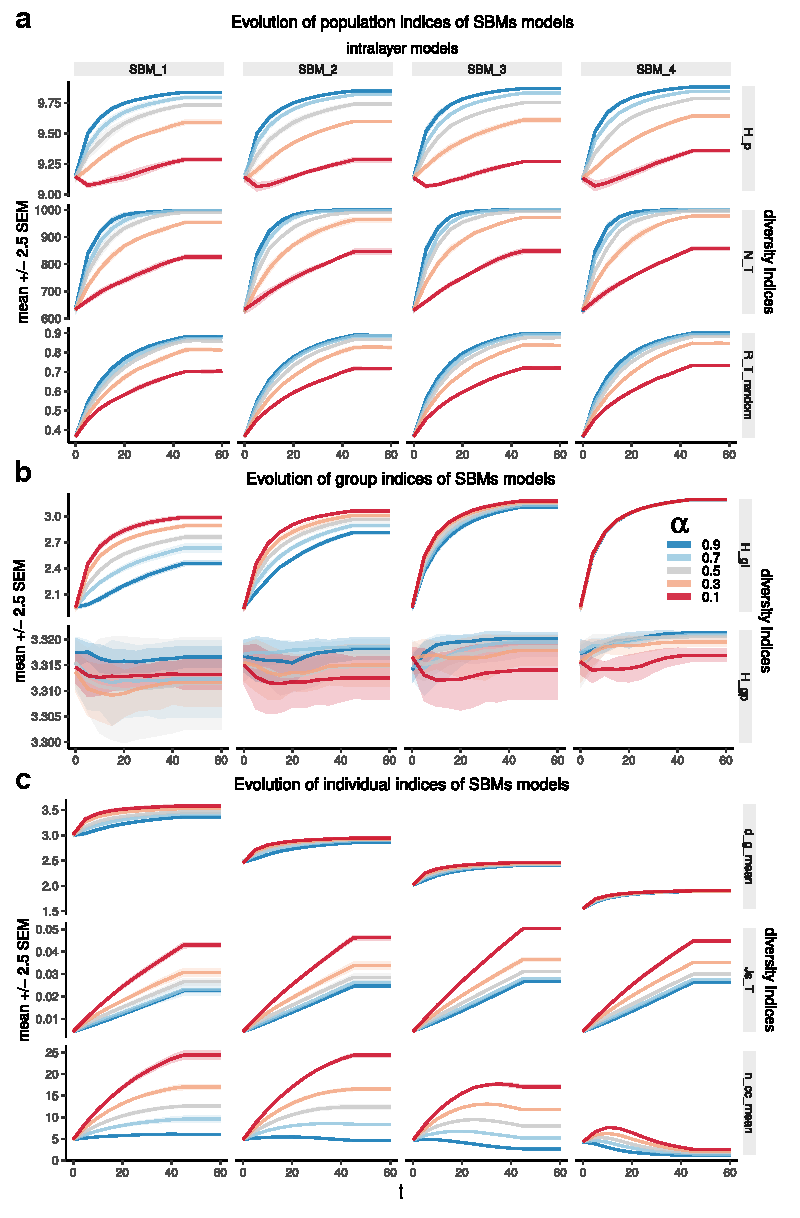
\includegraphics[width=\textwidth]{figures/FigS3.pdf}
    \caption{\label{fig:6}
    \textit{Summary  of  population  and  individual  diversity  indices  due  to $\alpha$,  across  different  block  models}. Within each panel, x-axis shows decreasing modularity of intralayer model, y-axis is $\alpha$ while the color represents values here at the end of the simulation, and min-max normalized within each metric. From left to right are different diversity metrics (see text for more information). From top to bottom are different group correspondence initialization strategies (top is equivalent to a random initialization; see \ref{supp:2} for example)
    }
\end{figure}